Este capítulo apresenta os conceitos fundamentais que sustentam o desenvolvimento deste trabalho. Aborda-se a problemática da navegação autônoma em robótica móvel, a definição formal do algoritmo SLAM (\textit{Simultaneous Localization and Mapping}), com ênfase na abordagem visual (vSLAM), e a arquitetura típica de processamento desses sistemas.

\section{Robótica Móvel e Navegação Autônoma}

Robôs móveis autônomos são sistemas mecânicos inteligentes projetados para navegar e executar tarefas em seus ambientes operacionais sem intervenção humana direta, exigindo a capacidade de tomar decisões com base em dados sensoriais incertos \cite{taheri2021slamdefinitionevolution, cadena2016presentfuturesimultaneous}. A capacidade de se mover de forma independente em um espaço desconhecido ou dinâmico é uma das competências mais críticas para robôs de serviço, demandando a integração robusta de múltiplos sistemas de hardware e software \cite{araujo2023atmosbotpropostamodelagem}.

A navegação autônoma não se resume apenas à locomoção; ela é o resultado de um ciclo contínuo de processamento de informações. Segundo \citeonline{araujo2023atmosbotpropostamodelagem}, a navegação bem-sucedida depende de quatro tarefas fundamentais:
\begin{enumerate}
    \item \textbf{Percepção:} A coleta de dados do ambiente através de sensores (ex.: câmeras, LiDAR (\textit{Light Detection and Ranging}) e unidades de medição inercial (IMU, do inglês \textit{Inertial Measurement Unit})) para extrair informações relevantes sobre o espaço físico;
    \item \textbf{Localização:} A capacidade do robô de estimar sua própria posição e orientação (pose) dentro de um sistema de coordenadas global ou local.
    \item \textbf{Planejamento:} A elaboração de uma trajetória segura e eficiente do ponto atual até o objetivo desejado, considerando obstáculos estáticos e dinâmicos.
    \item \textbf{Controle de Locomoção:} A atuação nos motores e rodas para executar fisicamente a trajetória planejada, corrigindo desvios em tempo real.
\end{enumerate}

Para que esse ciclo funcione em ambientes onde não se possui um mapa prévio (ambientes desconhecidos), o robô precisa resolver simultaneamente a localização e o mapeamento, uma interdependência que constitui o cerne do problema de SLAM \cite{taheri2021slamdefinitionevolution}.


\section{O Problema do SLAM}

O SLAM (\textit{Simultaneous Localization and Mapping}) é a técnica computacional que permite a um robô ou dispositivo móvel construir um mapa de um ambiente desconhecido e, simultaneamente, estimar sua trajetória dentro deste mapa \cite{taheri2021slamdefinitionevolution}. Este processo é frequentemente descrito na literatura como um problema do ``ovo e da galinha'': para construir um mapa preciso, o robô necessita de uma estimativa exata de sua localização; contudo, para se localizar com precisão, ele necessita de um mapa prévio do ambiente \cite{lemos2019plataformaroboticamovel, guapacha2017localizacaomapeamentosimultaneos}.

Do ponto de vista probabilístico, o SLAM trata de estimar a distribuição de probabilidade conjunta da trajetória do robô e da estrutura do mapa, dados os comandos de controle (movimento) e as observações dos sensores. Essa abordagem estatística é necessária porque tanto a odometria do robô quanto as medidas dos sensores são sujeitas a erros e ruídos, que, se não tratados, levariam a uma divergência rápida na estimativa da posição \cite{guapacha2017localizacaomapeamentosimultaneos, taheri2021slamdefinitionevolution}.

A literatura moderna, consolidada por \citeonline{cadena2016presentfuturesimultaneous}, divide a arquitetura de um sistema SLAM em dois componentes principais que operam de forma complementar:

\begin{itemize}
    \item \textbf{Front-end (Processamento Sensorial):} É a camada de abstração do sensor. Responsável por processar os dados brutos (como imagens ou nuvens de pontos) para extrair características relevantes e realizar a associação de dados (\textit{data association}) entre medições consecutivas. O \textit{front-end} gera restrições geométricas relativas, fornecendo uma estimativa inicial da trajetória do robô (odometria) \cite{cadena2016presentfuturesimultaneous, jin2019visualslamrgbd}.
    
    \item \textbf{Back-end (Otimização Global):} Responsável pela consistência global do sistema. Ele recebe as restrições geradas pelo \textit{front-end} e realiza a otimização do grafo de poses (\textit{Pose Graph Optimization}) ou ajuste de feixes (\textit{Bundle Adjustment}) para minimizar o erro acumulado (\textit{drift}). Uma função crítica do \textit{back-end} é gerenciar o fechamento de ciclo (\textit{loop closure}), corrigindo deformações na trajetória quando o robô revisita uma área conhecida \cite{cadena2016presentfuturesimultaneous, labbé2019rtabmapopensourcelidar}.
\end{itemize}

O processamento realizado pelo SLAM é baseado em elementos sensores que fornecem dados brutos sobre o ambiente. Estes sensores são denominados, no contexto de SLAM, como sensores de percepção.

\section{Sensores de Percepção para SLAM}

A escolha do sensor de percepção é uma decisão de projeto primária em sistemas de navegação, pois define a natureza dos dados que o algoritmo de SLAM deverá processar. Essa escolha envolve um compromisso (\textit{trade-off}) direto entre a riqueza de informações obtidas e o custo computacional para processá-las \cite{taheri2021slamdefinitionevolution}. Enquanto sensores a laser oferecem alta precisão geométrica com custo de processamento relativamente baixo, câmeras fornecem informações visuais densas, mas tendem a exigir maior poder de cálculo \cite{gatesichapakorn2019rosbasedautonomous}. Atualmente, os sensores mais comuns para esta tarefa são o LiDAR e as câmeras RGB-D \cite{jin2019visualslamrgbd, taheri2021slamdefinitionevolution}.

Entre os sensores a laser, o LiDAR é um sensor ativo que opera emitindo pulsos de luz (laser) e medindo o tempo de retorno para calcular a distância até os objetos. Essa tecnologia gera medições de alta precisão e longo alcance, sendo frequentemente considerada referência para mapeamento geométrico \cite{balado2025systematicliteraturereview}.

Em robótica móvel de baixo custo, é comum o uso de LiDARs 2D, que realizam uma varredura em um único plano horizontal. Embora eficientes para construir mapas de ocupação simples, esses sensores apresentam uma limitação crítica: a incapacidade de detectar obstáculos acima ou abaixo da linha do laser, como tampos de mesa ou degraus negativos, o que pode comprometer a segurança da navegação \cite{gatesichapakorn2019rosbasedautonomous}.

Por outro lado, LiDARs 3D (que geram nuvens de pontos volumétricas) possuem custo proibitivo para aplicações de serviço massificadas, sendo frequentemente classificados como soluções de ``grau de pesquisa'' (\textit{survey-grade}) \cite{balado2025systematicliteraturereview}. O trabalho de \citeonline{araujo2023atmosbotpropostamodelagem}, utilizado como base comparativa nesta pesquisa, adota a abordagem baseada em LiDAR, o que serve de contraponto para a avaliação da abordagem visual proposta aqui.

Como alternativa econômica e rica em informações, as câmeras RGB-D (\textit{Red, Green, Blue - Depth}) ganharam popularidade com o advento de dispositivos como o Microsoft Kinect \cite{microsoft2012kinect_v1} e o Asus Xtion \cite{asus2012xtionpro}. Estes sensores fornecem, simultaneamente, uma imagem colorida (RGB) e um mapa de profundidade (D), onde cada pixel contém a informação de distância do sensor até o objeto, permitindo uma percepção tridimensional densa do ambiente sem a complexidade mecânica de um LiDAR \cite{guapacha2017localizacaomapeamentosimultaneos}.

Existem duas tecnologias principais para a obtenção de profundidade em câmeras RGB-D, conforme detalhado por \citeonline{jin2019visualslamrgbd}:

\begin{enumerate}
    \item \textbf{Luz Estruturada (\textit{Structured Light}):} O sensor projeta um padrão conhecido de luz infravermelha (IR) no ambiente (como uma grade de pontos). A distorção desse padrão ao atingir superfícies curvas ou distantes é analisada para calcular a profundidade. Esta tecnologia, utilizada no Kinect v1 \cite{microsoft2012kinect_v1}, oferece boa precisão a curtas distâncias, mas sofre interferência severa sob luz solar direta.
    \item \textbf{Tempo de Voo (\textit{Time-of-Flight - ToF}):} O sensor emite pulsos de luz IR e mede o tempo exato que a luz leva para ir até o objeto e retornar. Utilizada no Kinect v2 \cite{microsoft2014kinect_v2} e sensores mais modernos, esta tecnologia oferece maior alcance e precisão, sendo menos suscetível a ruídos em comparação à luz estruturada \cite{kulkarni2021visualslamcombined}.
\end{enumerate}

A principal vantagem da câmera RGB-D sobre câmeras monoculares tradicionais é a obtenção direta da escala métrica do ambiente, eliminando a necessidade de complexos algoritmos de estimativa de profundidade ou movimento inicial para triangulação. No entanto, o uso de sensores RGB-D em plataformas embarcadas, como o Raspberry Pi, introduz um gargalo crítico: o volume massivo de dados (nuvens de pontos densas) exige alta largura de banda e processamento intensivo, o que pode degradar o desempenho da navegação em tempo real se não houver otimização \cite{gatesichapakorn2019rosbasedautonomous}.

\begin{table}[H]
\centering
\caption{Comparativo entre sensores de percepção para navegação robótica.}
\label{tab:comparativo_sensores}
\begin{tabular}{|l|l|l|}
\hline
\textbf{Característica} & \textbf{LiDAR 2D} & \textbf{Câmera RGB-D} \\ \hline
Tipo de Dado & Distância planar (2D) & Imagem + Profundidade (3D) \\ \hline
Custo Financeiro & Médio/Alto & Baixo (Sensores de consumo) \\ \hline
Custo Computacional & Baixo & Alto (Processamento de Imagem) \\ \hline
Sensibilidade à Luz & Robusto (Ativo) & Sensível (especialmente IR) \\ \hline
Detecção de Obstáculos & Apenas na altura do laser & Volumétrica (3D) \\ \hline
\end{tabular}
\fonte{Elaborado pelo autor com base em \citeonline{gatesichapakorn2019rosbasedautonomous} e \citeonline{jin2019visualslamrgbd}.}
\end{table}

Apesar das vantagens de custo e riqueza de informação, o uso exclusivo de câmeras RGB-D em aplicações de mapeamento e navegação pode apresentar limitações físicas em comparação a sensores a laser. \citeonline{kamarudin2015improvingperformance2d} demonstram experimentalmente que o campo de visão (FOV) mais estreito e o alcance limitado de sensores RGB-D típicos (como o Kinect) podem resultar em mapas de menor qualidade em ambientes amplos ou em corredores longos com poucas características visuais distintas, cenários nos quais o LiDAR tradicionalmente apresenta desempenho superior.

Diante da escolha da câmera RGB-D como sensor principal, devido ao seu baixo custo e capacidade de percepção 3D, torna-se necessário adotar algoritmos de mapeamento capazes de processar informações visuais. Esta classe de algoritmos é denominada Visual SLAM.

\section{Visual SLAM (vSLAM)}
\label{sec:visual_slam}

Enquanto o SLAM tradicional pode utilizar diversos tipos de sensores, o Visual SLAM (vSLAM) refere-se especificamente à utilização de câmeras (monoculares, estéreo ou RGB-D) como fonte primária de percepção. Diferente dos sensores a laser (LiDAR), que fornecem diretamente a geometria do ambiente, as câmeras entregam uma projeção 2D de intensidade de luz, exigindo que o algoritmo extraia computacionalmente as informações geométricas e semânticas necessárias para a navegação \cite{jin2019visualslamrgbd, mokssit2023deeplearningtechniques}.

Para detalhar o funcionamento deste algoritmo, utiliza-se o fluxo de processamento proposto por \citeonline{mokssit2023deeplearningtechniques}. A Figura \ref{fig:vslam_pipeline} ilustra este \textit{pipeline}, que decompõe o problema complexo do SLAM em módulos funcionais sequenciais, desde a aquisição da imagem até a geração do mapa global consistente.

\begin{figure}[H]
    \centering
    \caption{Pipeline geral de um sistema de Visual SLAM: da extração de características à otimização global.}
    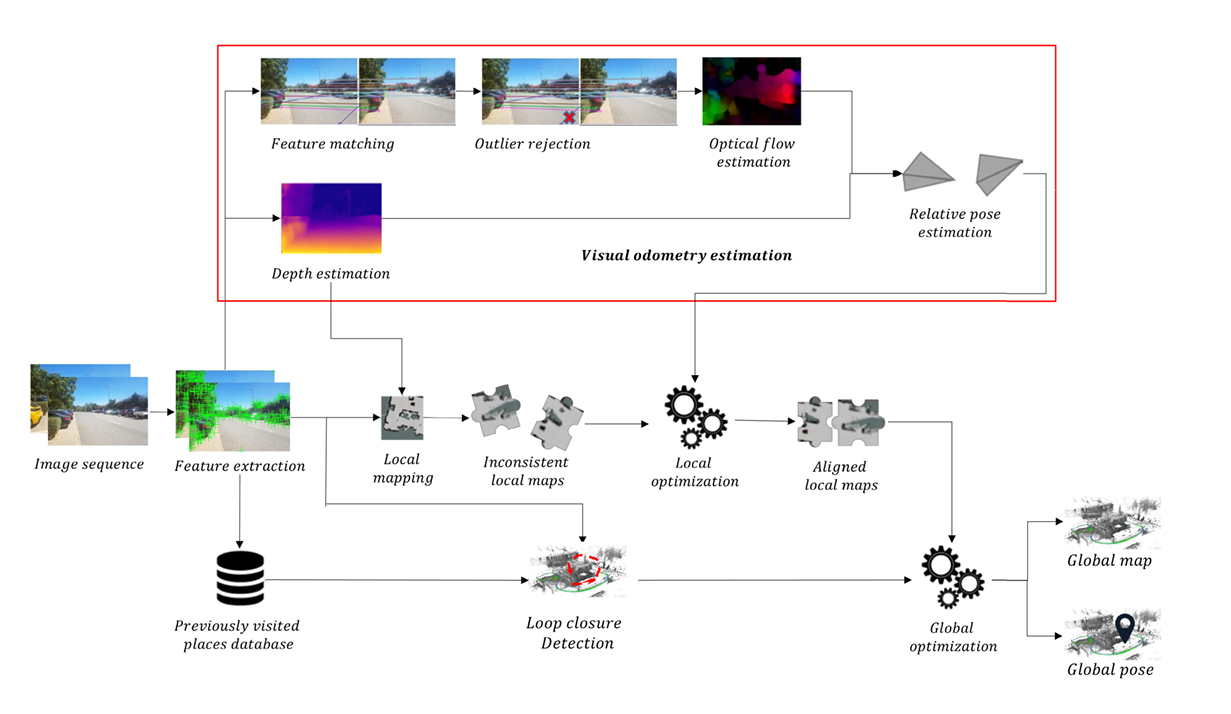
\includegraphics[width=1.0\textwidth]{figuras/vslam-pipeline.png}
    \fonte{\citeonline{mokssit2023deeplearningtechniques}.}
    \label{fig:vslam_pipeline}
\end{figure}

A seguir, detalham-se as etapas deste processo, relacionando-as com a arquitetura clássica de \textit{front-end} e \textit{back-end} discutida anteriormente.

\subsection{Extração de Características e Odometria Visual}

A primeira etapa, situada no \textit{Front-end} do sistema, lida com a percepção imediata do ambiente. Como câmeras convencionais não fornecem profundidade direta (diferente de sensores LiDAR que geram nuvens de pontos 3D imediatas), o algoritmo precisa processar a imagem 2D para extrair informações geométricas úteis.

A arquitetura de software adotada neste trabalho não visa reimplementar os componentes fundamentais do vSLAM, mas sim integrar e avaliar o desempenho de bibliotecas consolidadas, como o RTAB-Map, que encapsulam o fluxo de processamento descrito a seguir.

O processo inicia-se com a \textbf{Extração de Características}. O algoritmo identifica pontos de interesse na imagem (bordas, cantos e gradientes) e os descreve matematicamente. Algoritmos como o ORB (\textit{Oriented FAST and Rotated BRIEF}) são frequentemente utilizados nesta etapa por sua eficiência computacional em comparação a métodos mais pesados como SIFT ou SURF \cite{rublee2011orbefficientalternative, campos2021orbslam3accurateopensource}.

Com as características extraídas, entra em ação a \textbf{Odometria Visual (VO)}. Seu objetivo é estimar o movimento da câmera analisando como essas características mudam de posição entre quadros consecutivos. Conforme a literatura base \cite{scaramuzza2011visualodometrytutorial, mokssit2023deeplearningtechniques}, esta etapa é composta por componentes críticos:

\begin{itemize}
    \item \textbf{Correspondência de Características (\textit{Feature Matching}):} O sistema rastreia os pontos de interesse de um quadro para o outro, estabelecendo pares correspondentes.
    \item \textbf{Rejeição de Outliers:} Como a correspondência visual é propensa a erros (ruído ou texturas repetitivas), algoritmos estatísticos como o RANSAC são aplicados para descartar associações incorretas que degradariam a estimativa.
    \item \textbf{Estimativa de Pose e Profundidade:} Com base nas correspondências validadas, calcula-se a transformação geométrica (rotação e translação) da câmera. Em sistemas monoculares, a profundidade é estimada por triangulação; já em sistemas RGB-D, a profundidade é obtida diretamente do sensor, aumentando a precisão da odometria.
\end{itemize}

\subsection{Mapeamento e Otimização Local}

Enquanto a odometria fornece o movimento relativo instantâneo, o bloco de \textbf{Mapeamento Local} é responsável por projetar as características 2D rastreadas para o espaço 3D, criando uma representação espacial do ambiente ao redor do robô.

No entanto, a odometria visual acumula pequenos erros a cada quadro (\textit{drift}). Para mitigar isso, aplica-se a \textbf{Otimização Local}. O sistema mantém um "mapa local" (uma janela temporal recente de quadros e pontos) e realiza ajustes matemáticos, como o Ajuste de Feixes Local (\textit{Local Bundle Adjustment}). O objetivo é realinhar as poses da câmera e os pontos 3D para garantir que a trajetória local seja suave e consistente antes de ser integrada ao mapa global \cite{mur-artal2015orbslamversatileaccurate}.

\subsection{Fechamento de Ciclo e Otimização Global}

Os dois últimos blocos do fluxo correspondem ao \textit{Back-end} e lidam com a consistência do mapa em larga escala e longo prazo.

\begin{itemize}
    \item \textbf{Detecção de Fechamento de Ciclo (\textit{Loop Closure}):} Esta etapa permite que o robô reconheça lugares previamente visitados. Utilizando técnicas como \textit{Bag-of-Words}, o algoritmo compara a imagem atual com um banco de dados de imagens passadas. Se uma similaridade alta for detectada, o sistema entende que o robô "fechou um ciclo" \cite{mur-artal2015orbslamversatileaccurate}.
    
    \item \textbf{Otimização Global:} A detecção de um ciclo fornece uma forte restrição geométrica que conecta o início e o fim da trajetória (ou partes distantes dela). Algoritmos de Otimização de Grafos (\textit{Pose Graph Optimization}) utilizam essa informação para redistribuir o erro acumulado por todo o mapa, corrigindo a deriva e gerando uma representação globalmente coerente \cite{mokssit2023deeplearningtechniques}.
\end{itemize}

Embora o fluxo de processamento do vSLAM gere uma representação rica do ambiente e estime a trajetória da câmera, estes dados brutos não são, por si sós, suficientes para a autonomia do robô. Para se deslocar de forma inteligente, o sistema precisa traduzir essa percepção visual em informações de "ocupação" e "custo" compreensíveis para os algoritmos de controle de movimento. Isso nos conduz aos fundamentos da Navegação Autônoma.

\section{Navegação Autônoma}
\label{sec:navegacao}

A capacidade de um robô móvel deslocar-se de um ponto inicial até um objetivo de forma segura e eficiente, sem intervenção humana, define o problema da navegação autônoma. Em sistemas robóticos de serviço, essa tarefa não é trivial, pois exige a integração contínua entre a percepção do ambiente (mapas e sensores), a localização do robô e o controle dos atuadores (motores) \cite{macenski2020marathon2navigation}.

A arquitetura padrão para navegação em ambientes internos, consolidada pelo \textit{Navigation Stack} do ROS (\textit{Robot Operating System}), decompõe o problema em dois níveis hierárquicos de planejamento: o Planejamento Global e o Planejamento Local, ambos operando sobre representações do ambiente conhecidas como Mapas de Custo ou \textit{Costmaps} \cite{marder-eppstein2010officemarathonrobust}.

Para que o robô possa planejar caminhos seguros, o mapa métrico gerado pelo sistema de SLAM (descrito na seção anterior) precisa ser interpretado em termos de "custo de travessia". Segundo \citeonline{marder-eppstein2010officemarathonrobust}, o \textit{costmap} é uma grade de ocupação 2D onde cada célula possui um valor que indica a periculosidade daquela área.

Existem tipicamente dois tipos de \textit{costmaps} operando simultaneamente:
\begin{itemize}
    \item \textbf{Costmap Global:} Utiliza o mapa estático completo do ambiente (gerado previamente pelo SLAM) para planejar rotas longas.
    \item \textbf{Costmap Local:} É uma janela deslizante centrada no robô, atualizada em tempo real pelos sensores (como a câmera RGB-D ou LiDAR), permitindo a detecção de obstáculos dinâmicos que não existiam no mapa original, como pessoas ou móveis que mudaram de lugar \cite{macenski2020marathon2navigation}.
\end{itemize}

Uma característica crucial descrita por \citeonline{marder-eppstein2010officemarathonrobust} é a "inflação" dos obstáculos. Ao redor de cada obstáculo detectado, cria-se uma zona de segurança baseada no raio do robô, garantindo que o planejador nunca trace uma rota que passe perigosamente perto de uma parede ou objeto.

Com base nos mapas de custo, o sistema de navegação atua em dois estágios complementares:

\textbf{1. Planejador Global (\textit{Global Planner}):} Este módulo calcula a rota ideal de alto nível desde a posição atual do robô até o objetivo final. Utilizando algoritmos de busca em grafos, como o A* (\textit{A-Star}) ou Dijkstra, ele gera uma sequência de coordenadas (o caminho) que desvia dos obstáculos estáticos conhecidos no mapa \cite{marder-eppstein2010officemarathonrobust}. No entanto, este planejador não considera a cinemática do robô (velocidade, aceleração) nem obstáculos dinâmicos repentinos.

\textbf{2. Planejador Local (\textit{Local Planner}):} Responsável pela execução do movimento, o planejador local recebe o caminho global e gera comandos de velocidade linear e angular ($v, \omega$) para os motores do robô. Segundo \citeonline{macenski2020marathon2navigation}, este controlador deve reagir rapidamente a mudanças no ambiente.

Uma das abordagens mais utilizadas, descrita na arquitetura proposta por \citeonline{marder-eppstein2010officemarathonrobust}, é a simulação de trajetória (\textit{Trajectory Rollout}) ou a Janela Dinâmica (DWA). O algoritmo simula diversos caminhos possíveis para os próximos segundos, considerando as restrições físicas do robô (aceleração máxima), e seleciona aquele que maximiza o progresso em direção ao objetivo enquanto mantém uma distância segura de obstáculos detectados no \textit{costmap} local.

Portanto, no contexto deste trabalho, o sistema de Visual SLAM fornece a base necessária para etapas posteriores de navegação, ao estimar a pose e construir o mapa do ambiente. A integração completa com planejadores de trajetória, como os disponibilizados pelo Nav2, permanece como continuidade futura após a estabilização do mapeamento e da localização.

Conclui-se, portanto, que uma arquitetura de robótica de serviço eficiente necessita de um mediador robusto. É preciso um sistema capaz de executar o vSLAM para manter a localização precisa (Seção \ref{sec:visual_slam}), mas que também processe e projete eficientemente as informações 3D para alimentar os \textit{costmaps} 2D exigidos pela pilha de navegação (Seção \ref{sec:navegacao}). É neste contexto que o RTAB-Map se destaca como a solução escolhida para este trabalho.

\section{O Algoritmo RTAB-Map}
\label{sec:rtab_map}

O RTAB-Map (\textit{Real-Time Appearance-Based Mapping}) é uma solução de SLAM baseada em grafos projetada especificamente para lidar com o problema de mapeamento de longo prazo em tempo real. Diferente de outros algoritmos que podem sofrer com o crescimento linear do consumo de processamento à medida que o mapa aumenta, o RTAB-Map implementa uma estratégia de gerenciamento de memória inspirada no modelo cognitivo humano \cite{labbé2019rtabmapopensourcelidar}.

Para realizar o fechamento de ciclo (\textit{loop closure}), o RTAB-Map utiliza uma abordagem baseada em aparência, empregando um modelo \textit{Bag-of-Words} para comparar a assinatura visual da imagem atual com as imagens armazenadas no banco de dados. Quando uma correspondência é encontrada, o algoritmo adiciona uma restrição ao grafo de poses e executa uma otimização global (geralmente utilizando g2o ou GTSAM) para corrigir a deriva acumulada na odometria, garantindo a consistência topológica do mapa \cite{labbé2019rtabmapopensourcelidar}.

Segundo \citeonline{labbé2019rtabmapopensourcelidar}, a arquitetura do algoritmo divide o gerenciamento dos nós do mapa em três camadas de memória para manter o tempo de processamento limitado:

\begin{itemize}
    \item \textbf{Memória de Curto Prazo (STM - \textit{Short-Term Memory}):} É a porta de entrada do sistema, onde os dados mais recentes da odometria visual são armazenados e avaliados inicialmente.
    
    \item \textbf{Memória de Trabalho (WM - \textit{Working Memory}):} Mantém apenas os nós mais relevantes e frequentes para a localização atual e para a detecção de fechamento de ciclo. O tamanho da WM é fixo e configurável (por exemplo, definido por um limite de tempo ou quantidade de nós). Isso garante que o tempo de otimização do grafo permaneça constante, respeitando as restrições de tempo real do robô.
    
    \item \textbf{Memória de Longo Prazo (LTM - \textit{Long-Term Memory}):} Funciona como um banco de dados em disco (armazenamento secundário). Quando a WM atinge seu limite, os nós mais antigos ou menos relevantes são transferidos ("esquecidos") para a LTM, liberando memória RAM.
\end{itemize}

O aspecto crucial desta abordagem para robôs com recursos limitados reside na capacidade de \textbf{recuperação}. Quando o robô retorna a uma área previamente visitada, o algoritmo detecta a similaridade visual e "lembra" dos nós antigos, trazendo-os da LTM de volta para a WM. Isso permite o fechamento de ciclo e a correção do mapa global sem que seja necessário manter todo o histórico do ambiente carregado na memória RAM simultaneamente \cite{labbé2019rtabmapopensourcelidar}.

Além de seu gerenciamento de memória, o RTAB-Map possui módulos de construção de mapas 3D e recursos de integração com pilhas de navegação como o Nav2 (\textit{Navigation2}). Com esse conjunto, é possível converter o mapa 3D proveniente da câmera RGB-D em uma grade de ocupação 2D, permitindo que robôs equipados apenas com câmera forneçam informações compatíveis com algoritmos de navegação padrão, sem a necessidade de um LiDAR (\textit{Light Detection and Ranging}) físico \cite{labbé2019rtabmapopensourcelidar}.

Contudo, embora o gerenciamento de memória do RTAB-Map mitigue o uso de RAM ao longo do tempo, o custo computacional imediato para o processamento das imagens (extração de características e cálculo de profundidade) e a otimização do grafo ainda recai sobre a CPU. Em plataformas embarcadas onde o processador principal também deve gerenciar o sistema operacional, a comunicação de rede e o controle dos motores, essa carga de processamento pode se tornar proibitiva, exigindo uma análise cuidadosa das limitações do hardware.

\section{Computação Embarcada e Restrições de Hardware}

A execução de algoritmos complexos, como os associados ao vSLAM, em plataformas móveis exige uma análise criteriosa das limitações de hardware. O Raspberry Pi é um computador de placa única (SBC, do inglês \textit{Single-Board Computer}) que integra um \textit{System-on-Chip} (SoC) ou, em cenários similares, um \textit{Multiprocessor System-on-Chip} (MPSoC), no qual CPU, GPU e memória compartilham recursos em um único chip \cite{raspberrypi2019raspberrypi}. Embora ofereçam baixo custo e eficiência energética, essas plataformas podem apresentar limitações práticas para cargas intensivas em tempo real, como orçamento energético e térmico (\emph{thermal throttling}), capacidade de RAM e largura de banda de memória, exigindo ajustes de configuração e otimização \cite{costa2019characterizingpolybenchgpu, balado2025systematicliteraturereview}.

O processamento de fluxos RGB-D é particularmente oneroso. A execução simultânea da odometria visual (extração e correspondência de características) e da otimização do grafo de poses demanda ciclos de CPU intensivos e acesso rápido à memória. Segundo \citeonline{costa2019characterizingpolybenchgpu}, o desempenho nessas plataformas é altamente dependente da gestão térmica e da eficiência energética; o uso contínuo de todos os núcleos de processamento pode levar ao superaquecimento, resultando em redução forçada de frequência (\textit{thermal throttling}) e perda de quadros no mapeamento.

Além do processamento, a largura de banda interna e externa é um gargalo crítico. A transferência de nuvens de pontos densas e imagens de alta resolução pode saturar os barramentos de comunicação, exigindo algoritmos otimizados que reduzam a quantidade de dados trafegados sem comprometer a precisão da localização \cite{zheng2016multiframegraphmatching}.

A utilização de SBCs, como o Raspberry Pi, na robótica móvel apresenta desafios específicos que vão além do simples poder de processamento bruto. 

\begin{itemize}
    \item \textbf{Compartilhamento de Memória:} Em arquiteturas MPSoC (\textit{Multiprocessor System-on-Chip}), a CPU e a GPU frequentemente compartilham o mesmo barramento e banco de memória RAM. O processamento de nuvens de pontos densas pelo vSLAM compete diretamente com o sistema operacional e a comunicação de rede, podendo causar latência no acesso aos dados \cite{costa2019characterizingpolybenchgpu}.
    
    \item \textbf{Gerenciamento Térmico (\textit{Thermal Throttling}):} A execução contínua de algoritmos de visão computacional eleva rapidamente a temperatura do SoC. Para evitar danos, o hardware reduz automaticamente a frequência de operação (\textit{throttling}), o que resulta em uma queda abrupta na taxa de quadros (FPS) e pode levar à perda de rastreamento do robô \cite{costa2019characterizingpolybenchgpu, canovas2021onboarddynamicrgbd}.
    
     \item \textbf{Custo de Processamento de Filtros:} Câmeras de baixo custo sofrem com desfoque de movimento (\textit{motion blur}) durante deslocamentos rápidos. Para mitigar este efeito, avalia-se a necessidade da fusão sensorial com unidades de medição inercial (\textbf{IMU}, do inglês \emph{Inertial Measurement Unit}). Contudo, a implementação de filtros de fusão (como Filtros de Kalman Estendidos) adiciona uma carga computacional extra à CPU do SBC, competindo com o algoritmo principal de SLAM \cite{qayyum2017imuaidedrgbd}.
\end{itemize}

Portanto, a viabilidade do robô depende de encontrar um equilíbrio entre a precisão do algoritmo (como os parâmetros do RTAB-Map) e a capacidade física do hardware de sustentar essa carga por períodos prolongados \cite{nagarajan2024multiobjectiveoptimizationrtabmap}.

\section{Execução Embarcada e Observabilidade do Sistema}

Para lidar com as restrições de hardware apresentadas, o projeto de um sistema robótico deve definir quais componentes serão executados no próprio robô e como o seu comportamento será observado durante os testes. Em robôs de baixo custo, a execução embarcada prioriza autonomia e simplicidade operacional, mas exige atenção ao consumo de CPU, à memória, à frequência dos sensores e à estabilidade térmica.

No processamento embarcado (\textit{onboard computing}), os módulos de percepção, odometria, otimização e publicação de mapas são executados localmente na CPU do robô. Esta abordagem garante maior independência em relação à infraestrutura externa e é coerente com a proposta de uma plataforma de baixo custo, mas impõe sacrifícios práticos: pode ser necessário reduzir resolução, diminuir frequência de atualização, ajustar parâmetros do RTAB-Map ou simplificar etapas de processamento para manter operação em tempo real \cite{canovas2021onboarddynamicrgbd, costa2019characterizingpolybenchgpu}.

A observabilidade do sistema, por sua vez, depende de ferramentas externas de monitoramento, como terminais remotos e RViz, que permitem inspecionar tópicos, transformações e mapas durante os ensaios. Essa observação externa não implica transferir o processamento principal do SLAM para outro computador; trata-se de um recurso de depuração, registro e análise do comportamento do robô físico.

Embora arquiteturas de processamento remoto ou \textit{offloading} sejam discutidas na literatura como alternativa para tarefas computacionalmente intensivas \cite{li2021highefficientmultirobot}, elas introduzem dependência de rede, latência variável, perda de pacotes e necessidade de alta largura de banda para fluxos RGB-D \cite{zheng2016multiframegraphmatching}. Por essa razão, nesta versão do trabalho, o \textit{offloading} não é tratado como eixo de validação. O foco recai sobre a execução embarcada no Raspberry Pi e sobre a identificação dos limites práticos dessa escolha.

Assim, a avaliação do artefato deve considerar não apenas se o mapa é produzido, mas se o pipeline mantém frequência, sincronização e transformações coerentes enquanto opera sob as restrições reais do hardware físico.

\section{Ferramentas de Desenvolvimento}

O desenvolvimento de sistemas robóticos complexos é facilitado por um ecossistema de software que permite modularização, comunicação, visualização e integração de sensores e atuadores, conforme apresentado nesta seção.

O ROS (\textit{Robot Operating System}) atua como um middleware de código aberto, fornecendo serviços que se esperaria de um sistema operacional, como abstração de hardware, controle de dispositivos de baixo nível, implementação de funcionalidades comumente usadas, passagem de mensagens entre processos e gerenciamento de pacotes \cite{quigley2009rosopensource}.

A arquitetura do ROS é baseada em um grafo de computação, onde o processamento ocorre em processos chamados ``nós'' (\textit{nodes}) que podem receber, postar e multiplexar mensagens de sensores, controle, estado, planejamento e atuadores. A comunicação ocorre através de ``tópicos'' (\textit{topics}) para fluxo de dados contínuo ou ``serviços'' (\textit{services}) para requisições síncronas. No ROS 2, a descoberta e a troca de mensagens são apoiadas por implementações DDS, dispensando o mestre central utilizado no ROS 1. A Figura \ref{fig:ros_architecture} ilustra, de forma geral, a comunicação entre nós e tópicos no ecossistema ROS.

\begin{figure}[H]
    \centering
    \caption{Arquitetura do sistema ROS e comunicação entre nós.}
    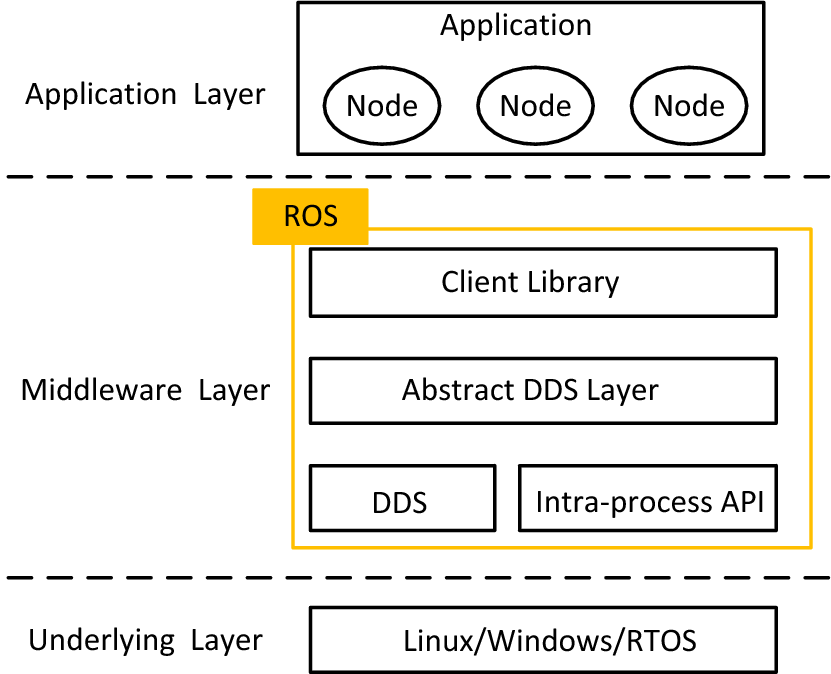
\includegraphics[width=0.8\textwidth]{figuras/ROS-architecture.png}
    \fonte{Adaptado de \citeonline{cui2019verifying}.}
    \label{fig:ros_architecture}
\end{figure}

O ROS simplifica o acesso ao hardware e oferece um vasto repositório de pacotes prontos, como o próprio RTAB-Map, permitindo o desenvolvimento modular e independente de drivers e algoritmos \cite{araujo2023atmosbotpropostamodelagem}.

O Gazebo é um simulador 3D robusto projetado para robótica, capaz de simular robôs, sensores e objetos em um ambiente tridimensional. Ele integra uma \textit{Physics Engine} para simular dinâmica e colisões, e um motor de renderização para gerar dados visuais realistas para as câmeras do robô \cite{koenig2004designuseparadigms}.

A arquitetura do Gazebo segue um modelo cliente-servidor, conforme ilustrado na Figura \ref{fig:gazebo_architecture}. O servidor (\textit{gzserver}) executa a física e a geração de dados dos sensores, enquanto o cliente (\textit{gzclient}) fornece a interface gráfica para o usuário. A comunicação com o ROS é realizada através do pacote \texttt{gazebo\_ros\_pkgs}, que permite que o robô simulado publique dados de sensores e receba comandos de velocidade nos mesmos tópicos que o robô real utilizaria, facilitando a transição da simulação para o hardware físico \cite{araujo2023atmosbotpropostamodelagem}.

\begin{figure}[h]
    \centering
    \caption{Estrutura e componentes da arquitetura do Gazebo.}
    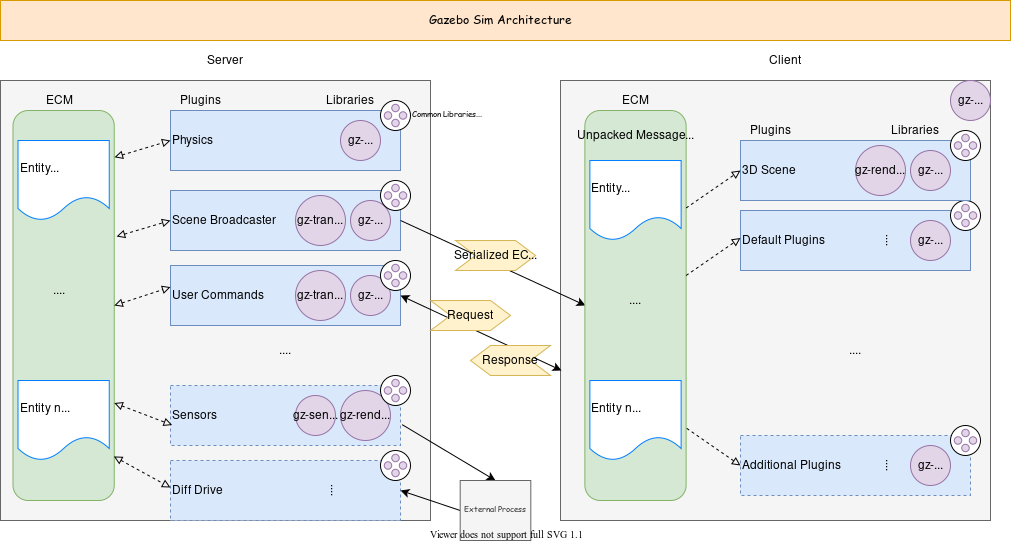
\includegraphics[width=0.8\textwidth]{figuras/GazeboSimArchitecture.png}
    \fonte{Adaptado de \citeonline{gazebo_architecture}.}
    \label{fig:gazebo_architecture}
\end{figure}

A simulação no Gazebo é uma ferramenta útil na robótica para testar lógica de navegação e integração entre componentes em ambiente seguro e controlado. Contudo, nesta versão do trabalho, ela não constitui o eixo de validação. A avaliação principal ocorre no hardware real, pois limitações de driver da câmera RGB-D, ruído efetivo dos sensores, comportamento da odometria e desempenho de CPU em tempo real só podem ser observados adequadamente no protótipo físico.
